% Editable native annotations around unchanged verified IDE photographs.
\par
\begin{figure}[htbp]
\centering
\sbox0{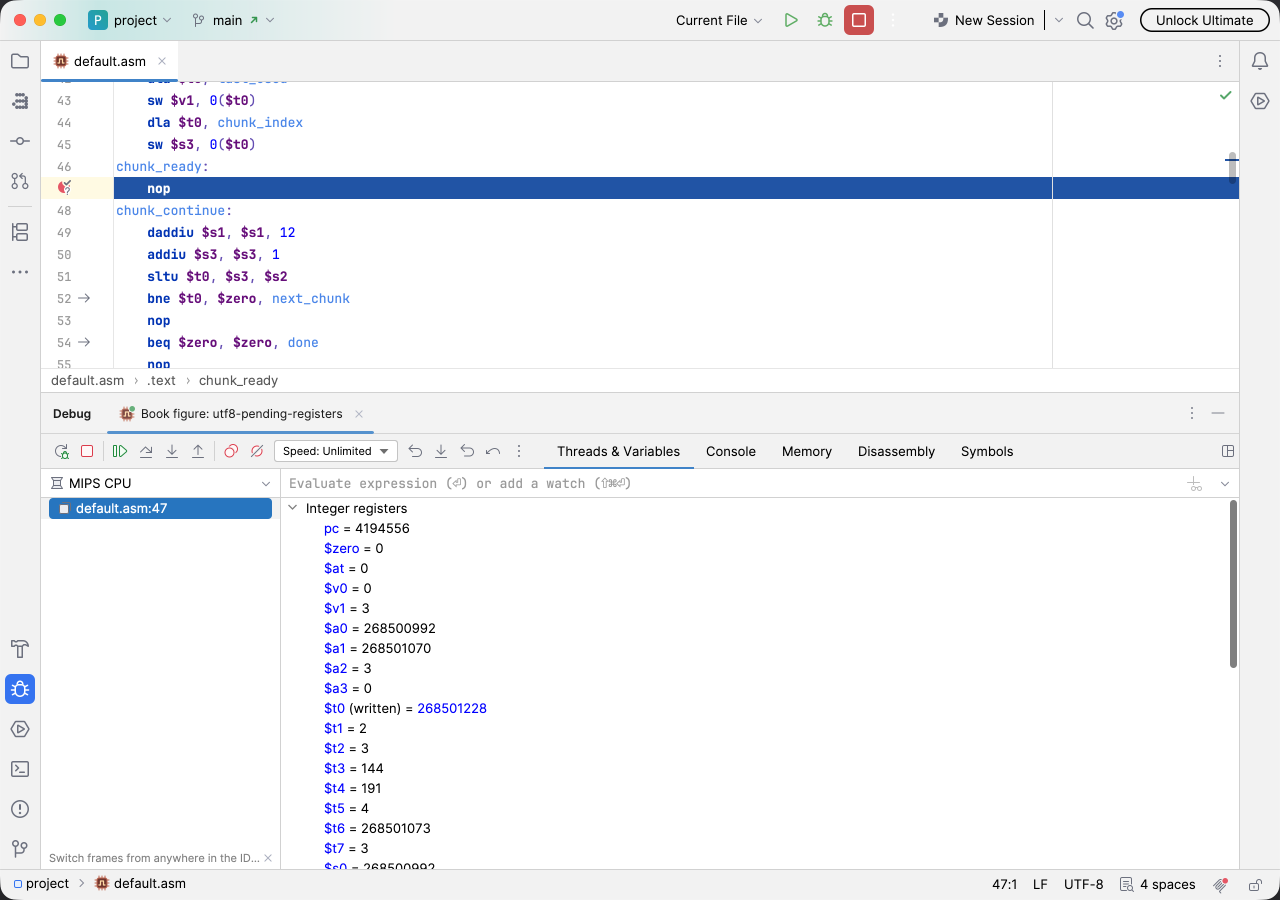
\includegraphics[artifact]{packages/015-utf8-scanner/captures/f01-pending/registers.png}}
\sbox2{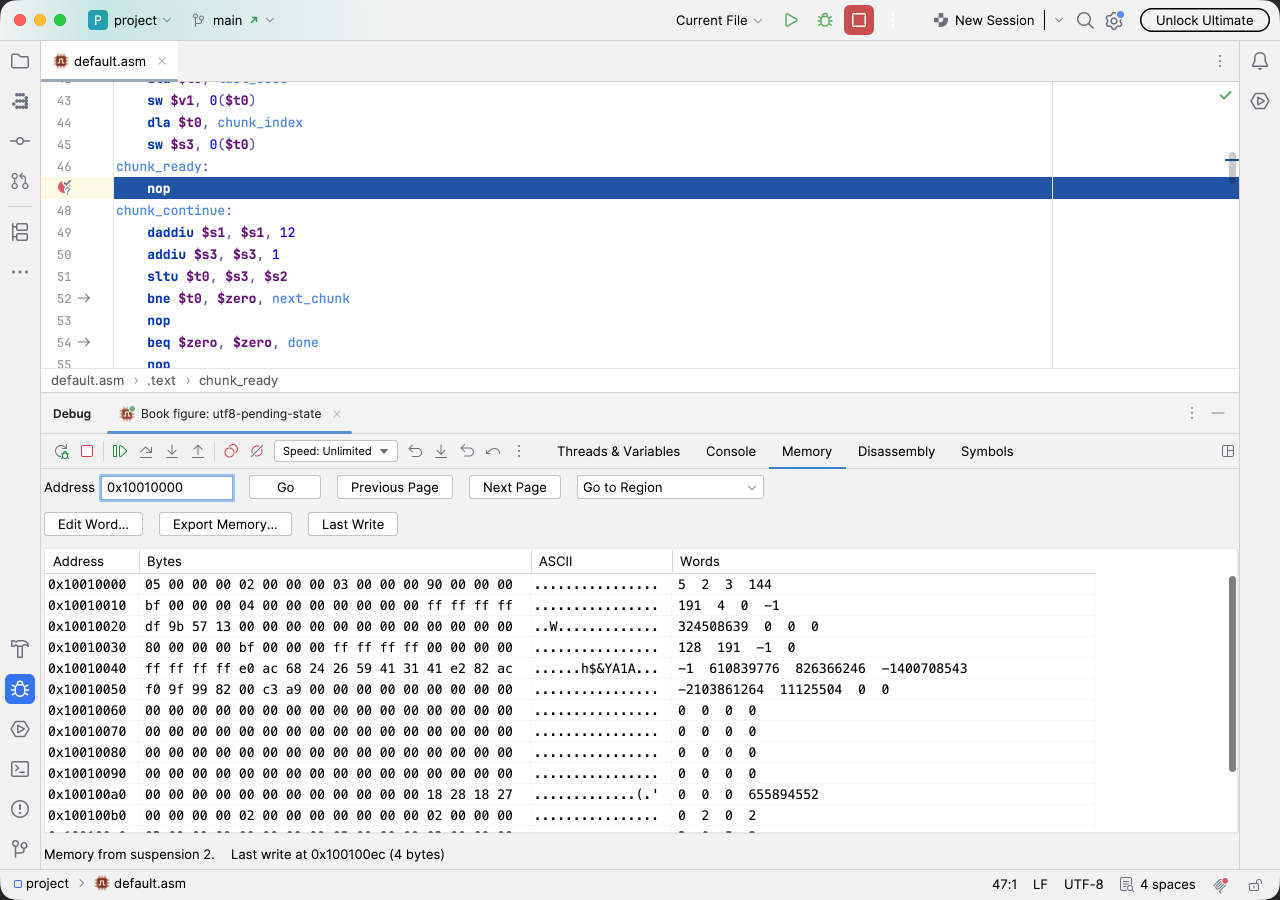
\includegraphics[artifact]{packages/015-utf8-scanner/captures/f01-pending/state.png}}
\sbox4{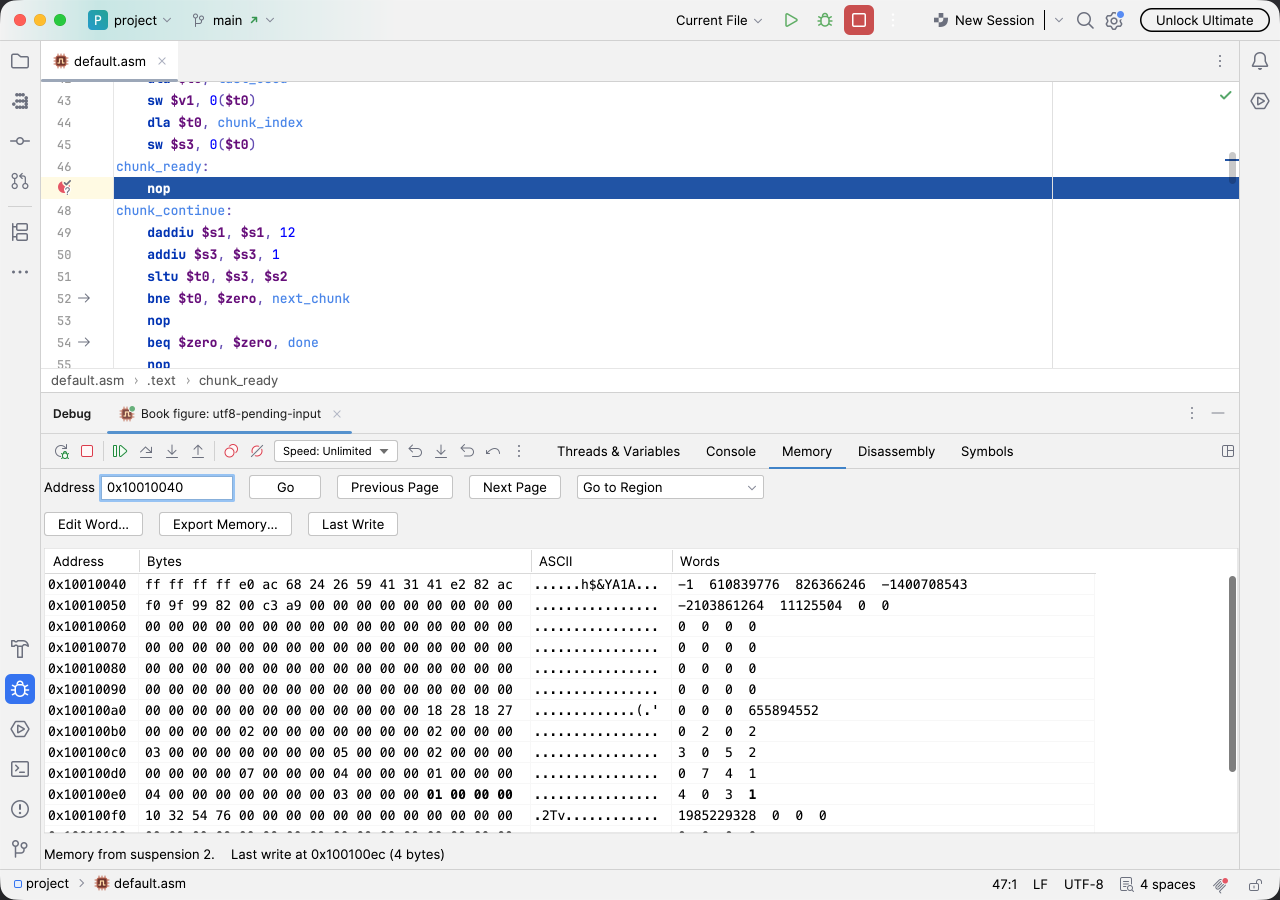
\includegraphics[artifact]{packages/015-utf8-scanner/captures/f01-pending/input.png}}
\edef\MARSutfpendingsourceLeft{\the\dimexpr0.036718750\wd0\relax}
\edef\MARSutfpendingsourceBottom{\the\dimexpr0.774444444\ht0\relax}
\edef\MARSutfpendingsourceRight{\the\dimexpr0.713281250\wd0\relax}
\edef\MARSutfpendingsourceTop{\the\dimexpr0.147777778\ht0\relax}
\edef\MARSutfpendingregistersLeft{\the\dimexpr0.246093750\wd0\relax}
\edef\MARSutfpendingregistersBottom{\the\dimexpr0.312222222\ht0\relax}
\edef\MARSutfpendingregistersRight{\the\dimexpr0.553906250\wd0\relax}
\edef\MARSutfpendingregistersTop{\the\dimexpr0.640000000\ht0\relax}
\edef\MARSutfpendingstateLeft{\the\dimexpr0.034375000\wd2\relax}
\edef\MARSutfpendingstateBottom{\the\dimexpr0.311111111\ht2\relax}
\edef\MARSutfpendingstateRight{\the\dimexpr0.584375000\wd2\relax}
\edef\MARSutfpendingstateTop{\the\dimexpr0.608888889\ht2\relax}
\edef\MARSutfpendinginputLeft{\the\dimexpr0.034375000\wd4\relax}
\edef\MARSutfpendinginputBottom{\the\dimexpr0.311111111\ht4\relax}
\edef\MARSutfpendinginputRight{\the\dimexpr0.584375000\wd4\relax}
\edef\MARSutfpendinginputTop{\the\dimexpr0.608888889\ht4\relax}
\begin{tikzpicture}[alt={Four annotated details after chunk index one. Native return status zero and used three accompany state total five, complete scalar count two, need three, low 144, high 191, start four, active status zero and error minus one. The input has A, euro bytes e2 82 ac and lead f0 across the first two calls. Three continuation bytes are still required.}]
\node[anchor=north west,inner sep=0,font=\small\bfseries] (source-title) at (6mm,0) {Next instruction after publication};
\node[anchor=north west,inner sep=0] (source) at ([yshift=-1mm]source-title.south west) {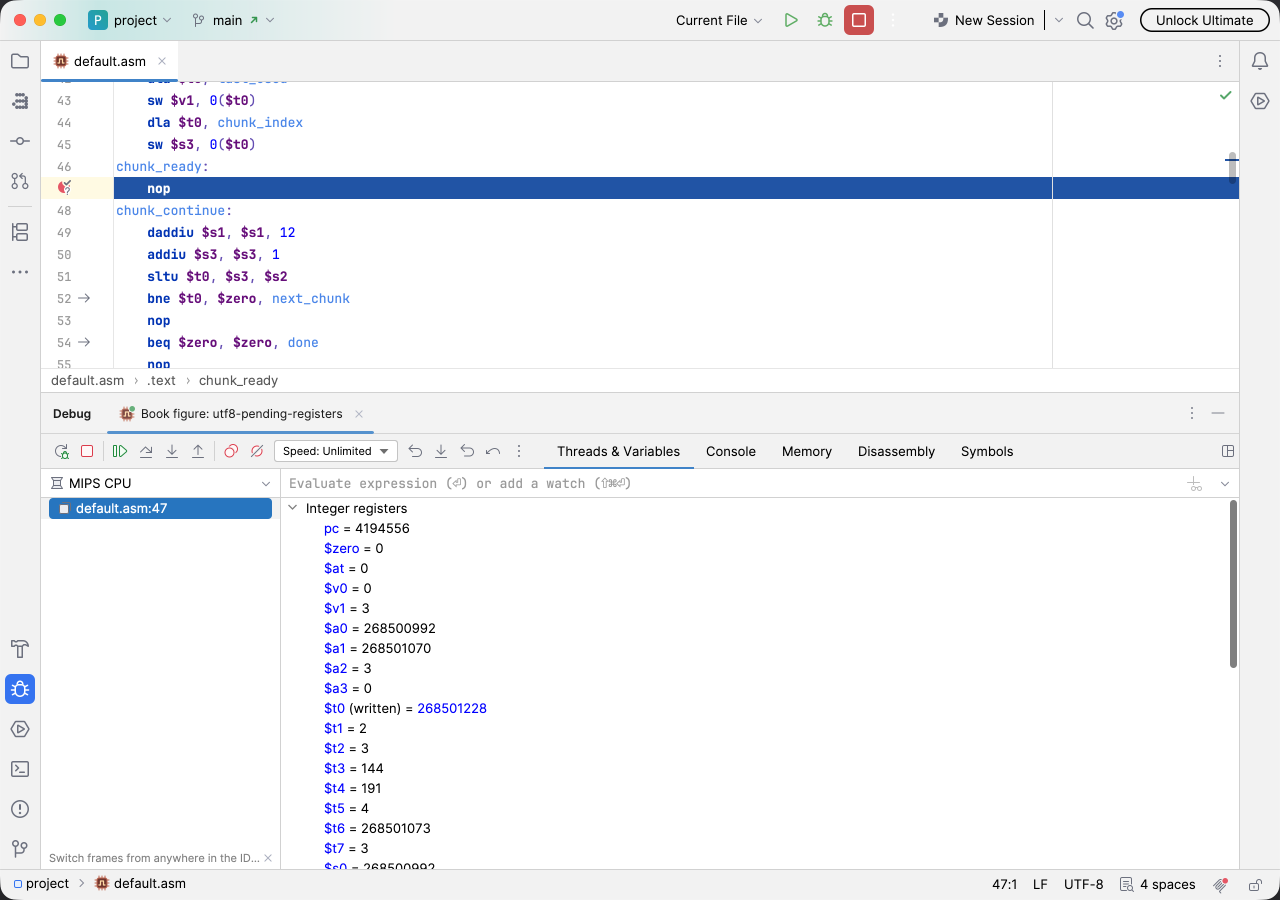
\includegraphics[width=0.54\linewidth,artifact,trim={\MARSutfpendingsourceLeft{} \MARSutfpendingsourceBottom{} \MARSutfpendingsourceRight{} \MARSutfpendingsourceTop{}},clip]{packages/015-utf8-scanner/captures/f01-pending/registers.png}};
\begin{scope}[shift={(source.south west)},x={($(source.south east)-(source.south west)$)},y={($(source.north west)-(source.south west)$)}]
\draw[black,line width=0.7pt] (0.215625000,0.057142857) rectangle (0.384375000,0.371428571);
\node[draw=black,fill=white,circle,inner sep=1.5pt,font=\footnotesize] at ($(0.215625000,0.371428571)+(-3mm,0)$) {1};
\end{scope}
\node[anchor=north west,inner sep=0,font=\small\bfseries] (registers-title) at (0.58\linewidth,0 |- source-title.north) {Signed return values};
\node[anchor=north west,inner sep=0] (registers) at ([yshift=-1mm]registers-title.south west) {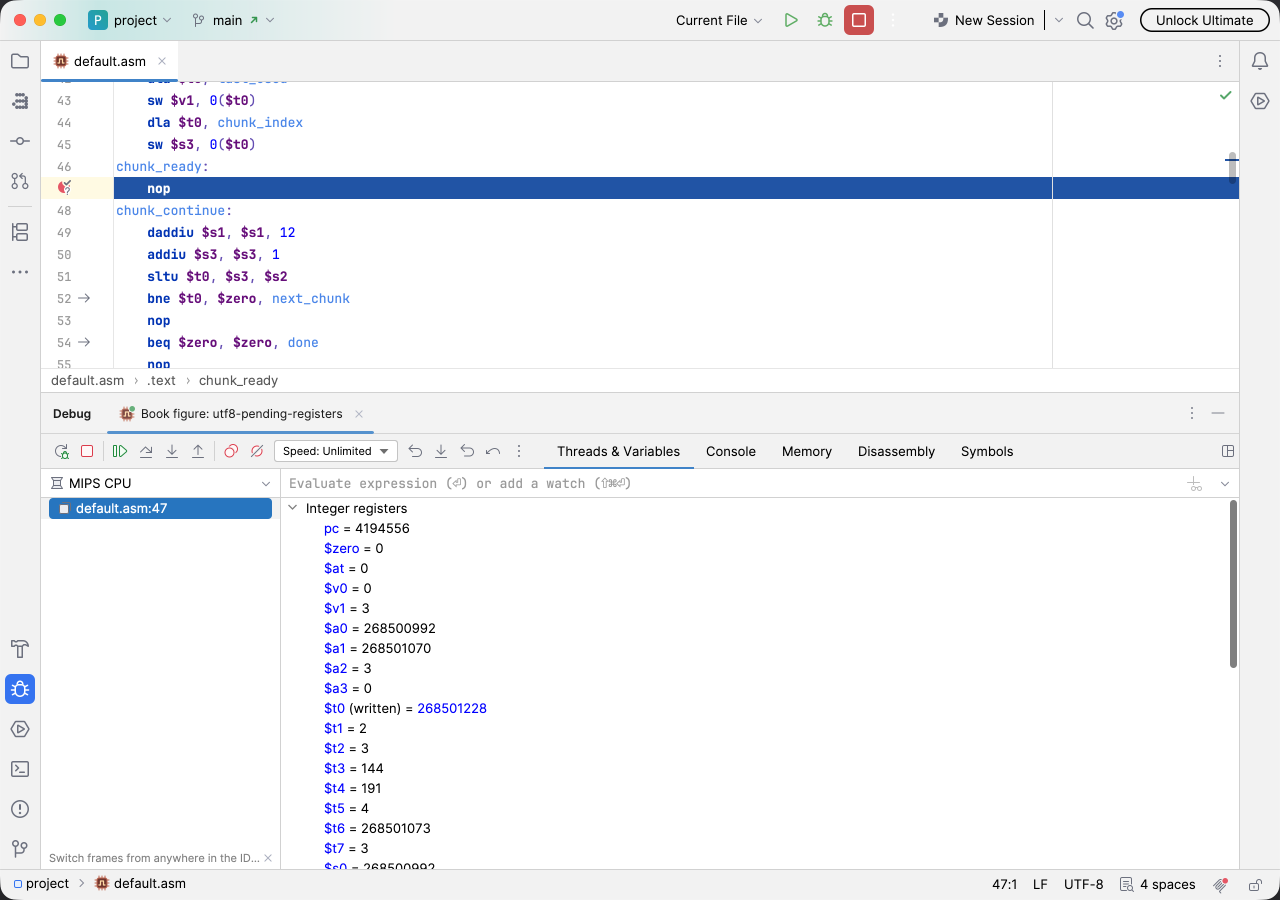
\includegraphics[width=0.42\linewidth,artifact,trim={\MARSutfpendingregistersLeft{} \MARSutfpendingregistersBottom{} \MARSutfpendingregistersRight{} \MARSutfpendingregistersTop{}},clip]{packages/015-utf8-scanner/captures/f01-pending/registers.png}};
\begin{scope}[shift={(registers.south west)},x={($(registers.south east)-(registers.south west)$)},y={($(registers.north west)-(registers.south west)$)}]
\draw[black,line width=0.7pt] (0.023437500,0.023255814) rectangle (0.226562500,0.953488372);
\node[draw=black,fill=white,circle,inner sep=1.5pt,font=\footnotesize] at ($(0.023437500,0.953488372)+(-3mm,0)$) {2};
\end{scope}
\node[anchor=north west,inner sep=0,font=\small\bfseries] (state-title) at ([yshift=-3mm]source.south west) {Stream state: eight little-endian words};
\node[anchor=north west,inner sep=0] (state) at ([yshift=-1mm]state-title.south west) {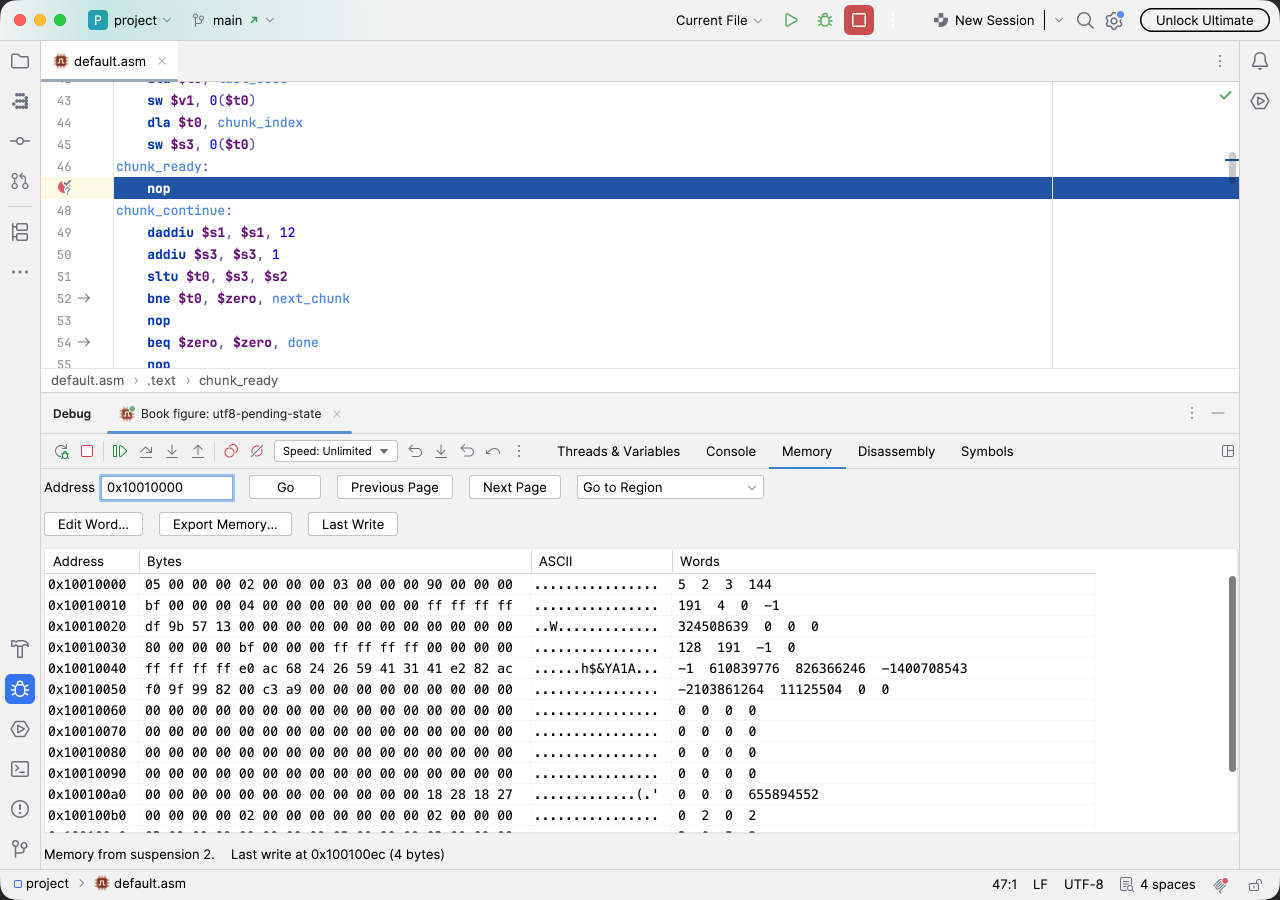
\includegraphics[width=0.84\linewidth,artifact,trim={\MARSutfpendingstateLeft{} \MARSutfpendingstateBottom{} \MARSutfpendingstateRight{} \MARSutfpendingstateTop{}},clip]{packages/015-utf8-scanner/captures/f01-pending/state.png}};
\begin{scope}[shift={(state.south west)},x={($(state.south east)-(state.south west)$)},y={($(state.north west)-(state.south west)$)}]
\draw[black,line width=0.7pt] (0.194672131,0.055555556) rectangle (0.997950820,0.638888889);
\node[draw=black,fill=white,circle,inner sep=1.5pt,font=\footnotesize] at ($(0,0.638888889)+(-3mm,0)$) {3};
\end{scope}
\node[anchor=north west,inner sep=0,font=\small\bfseries] (input-title) at ([yshift=-3mm]state.south west) {Mapped input and neighboring words};
\node[anchor=north west,inner sep=0] (input) at ([yshift=-1mm]input-title.south west) {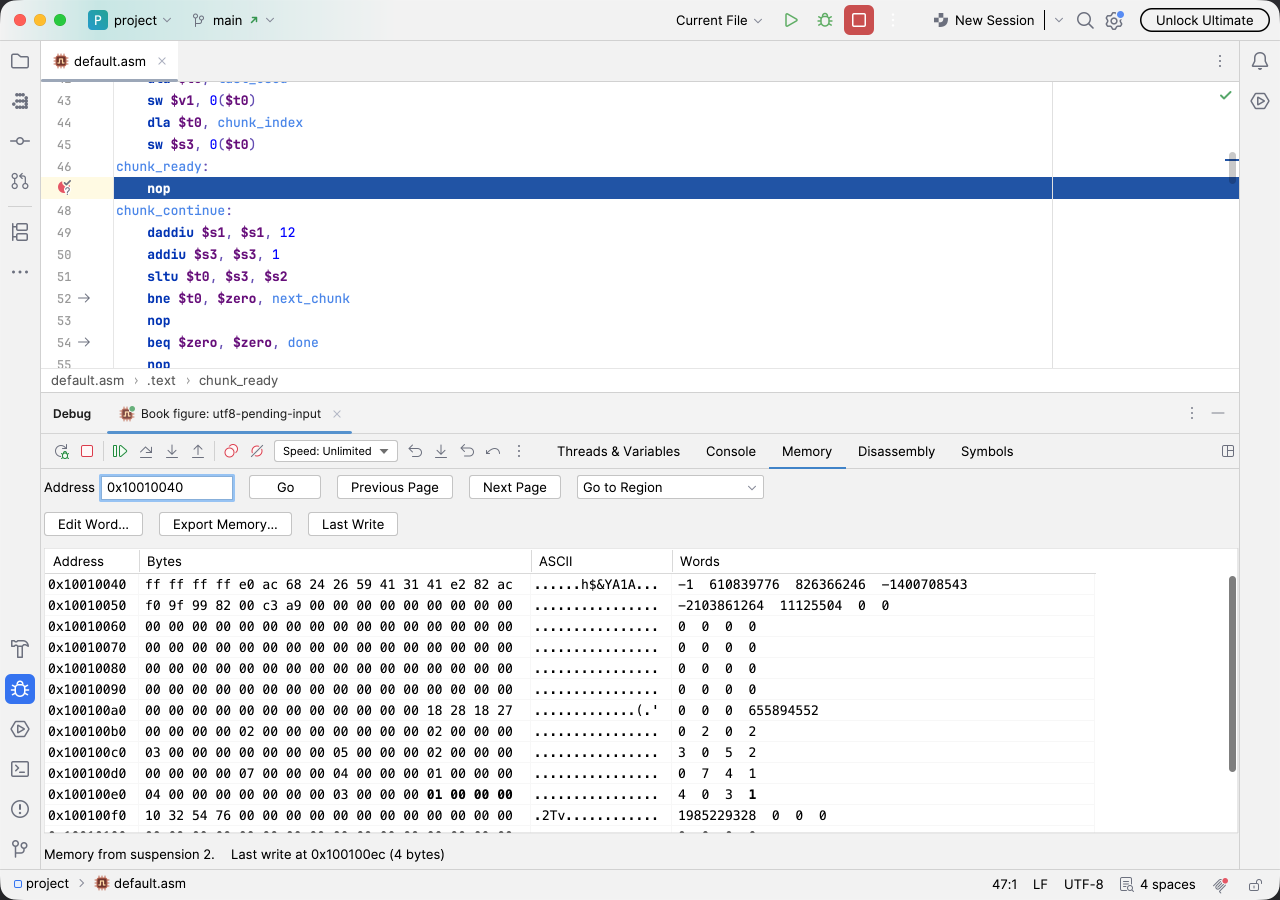
\includegraphics[width=0.84\linewidth,artifact,trim={\MARSutfpendinginputLeft{} \MARSutfpendinginputBottom{} \MARSutfpendinginputRight{} \MARSutfpendinginputTop{}},clip]{packages/015-utf8-scanner/captures/f01-pending/input.png}};
\begin{scope}[shift={(input.south west)},x={($(input.south east)-(input.south west)$)},y={($(input.north west)-(input.south west)$)}]
\draw[black,line width=0.7pt] (0.194672131,0.055555556) rectangle (0.997950820,0.638888889);
\node[draw=black,fill=white,circle,inner sep=1.5pt,font=\footnotesize] at ($(0,0.638888889)+(-3mm,0)$) {4};
\end{scope}
\end{tikzpicture}
\par\smallskip
\begin{minipage}{\linewidth}
\small
\begin{enumerate}
\setlength{\itemsep}{2pt}
\setlength{\parsep}{0pt}
\item The blue \texttt{nop} at \texttt{chunk\_ready} is next after chunk index 1, the second call. The scanner has returned and the caller has published its results. All panels replay the same fixture to the native conditional breakpoint \texttt{\$s3 == 1}.
\item The native signed-decimal view shows \texttt{\$v0 = 0}: the stream remains active. \texttt{\$v1 = 3} is the number of bytes accepted from this call, not the lifetime byte total or number of complete scalars. A non-final call may succeed while leaving a sequence pending.
\item The eight little-endian state words are $[5,2,3,144,191,4,0,-1]$. The first row holds total, count, need and low; the second holds high, start, status and error. Five bytes have been accepted, but only two scalar values are complete. Start 4 locates the pending lead in the stream; error $-1$ means no error has been reported.
\item The input begins at \texttt{0x1001004c}, twelve bytes into the first displayed row, with \texttt{41 e2 82 ac}. These encode \texttt{A} and U+20AC. The second call accepts \texttt{82 ac f0}: it completes U+20AC, then starts a four-byte sequence at stream offset 4. The next byte must be \texttt{90} through \texttt{bf}, decimal 144 through 191. Later bytes are mapped and visible, but belong to later calls.
\end{enumerate}
\end{minipage}
\caption{A four-byte lead remains pending after the second input chunk.}
\label{capture:015-utf8-scanner-f01-pending}
\label{utf8-f01-pending}
\end{figure}
\par
